\subsection{Project Management Summary}

\subsubsection{Time Management Record}

To effectively manage time over the course of the project the group constructed
a gannt chart to track the components tasks of the project and to fit those tasks into the
tight schedule defined by the project guidelines. To build the gantt chart the
group first plotted the milestones of the project (shown as diamonds on the
gantt chart); submitting a brief to the
customer, the two progress seminars, the report hand-in and the final
presentation. The time between the milestones formed the development cycles
used in the project, with two iterations of development of four weeks in length
each before each progress seminar. One week at the end of each iteration was
left for preparation of the progress seminar.

At the end of the first iteration, the group was on time with the deliverables
set in the plan, and there was time during the preparation of the first progress
seminar to integrate the code produced and present a demo of the framework
retrieving trends and URLs. After the progress seminar the group started work on
the malware scanners, having researched scanning methods during the first
iteration. When preparing for the second progress seminar, the group started to
suspect that the task of creating and integrating malware scanners into the
framework was harder than originally estimated, resulting in development effort
continuing after the second progress seminar in contrast to the plan. The
consequence of this was reduction in scope for the the amount of results
collected, and the delay of the web reporting interface to an additional task
completed after the delivery of the rest of the project but still in time for
presenting to the customer at the final presentation.

The Gantt charts can be found at the end of the project management summary.

\subsubsection{Writing the Report}

Although the first words of the report were written in early November, writing
the report started in earnest at the beginning of December. To aid the group
with assessing current progress with the report, a python script was written
that shows a day by day cumulative word count drawn on a stacked bar chart with
one segment per group member. The output of the python script is shown below.
This script uses the github API and texcount.pl script to count words in each
commit in the repository.

AWESOME REPORTIFICATE GRAPH

\subsubsection{Achievements \& Lessons Learnt}

The total length of time available to complete the project in was 11 weeks, in
this time the group had to fit in a customer brief, two presentations, and a
24000 word report. This meant that the effective development time for the
project was in the region of 4-6 weeks. In this time the group managed to
construct a working framework that could collect trends from a number of
sources, retrieve URLs related to those trends, and conduct rudimentary analysis
of the URLs for malware. As of writing the only working malware scanners are
those which involve the very lowest levels of interaction. Whilst the
Capture-HPC scanner was successfully integrated into the framework, further
configuration of the system is needed before it can be used to process URLs in
an effective way. The other malware scanners are not yet fully integrated into
the framework. Given the time constraints, the group managed to achieve most of
the work needed for a fully featured protoype and it is expected that it will be
possible to demo a completed version of the project at the final presentation to
the customer. In retrospect the scope of the project was very wide, and perhaps
a more complete product could have been delivered if the scope had been reduced
somewhat.

Another lession learned during the course of the project relates to the division
of work. The style of development was intended to allow a reasonable degree of
autonomy, but still provide ample opportunity for the group members to assit
each other with tasks in case of difficulty. An unintended consequence of this
was that no one group member had complete knowledge of all of the technical
aspects of the system, making integration more complicated and hence causing
delays.


\clearpage
\begin{landscape}
\subsection{Gantt Charts}
\begin{figure}[htb]
\centering
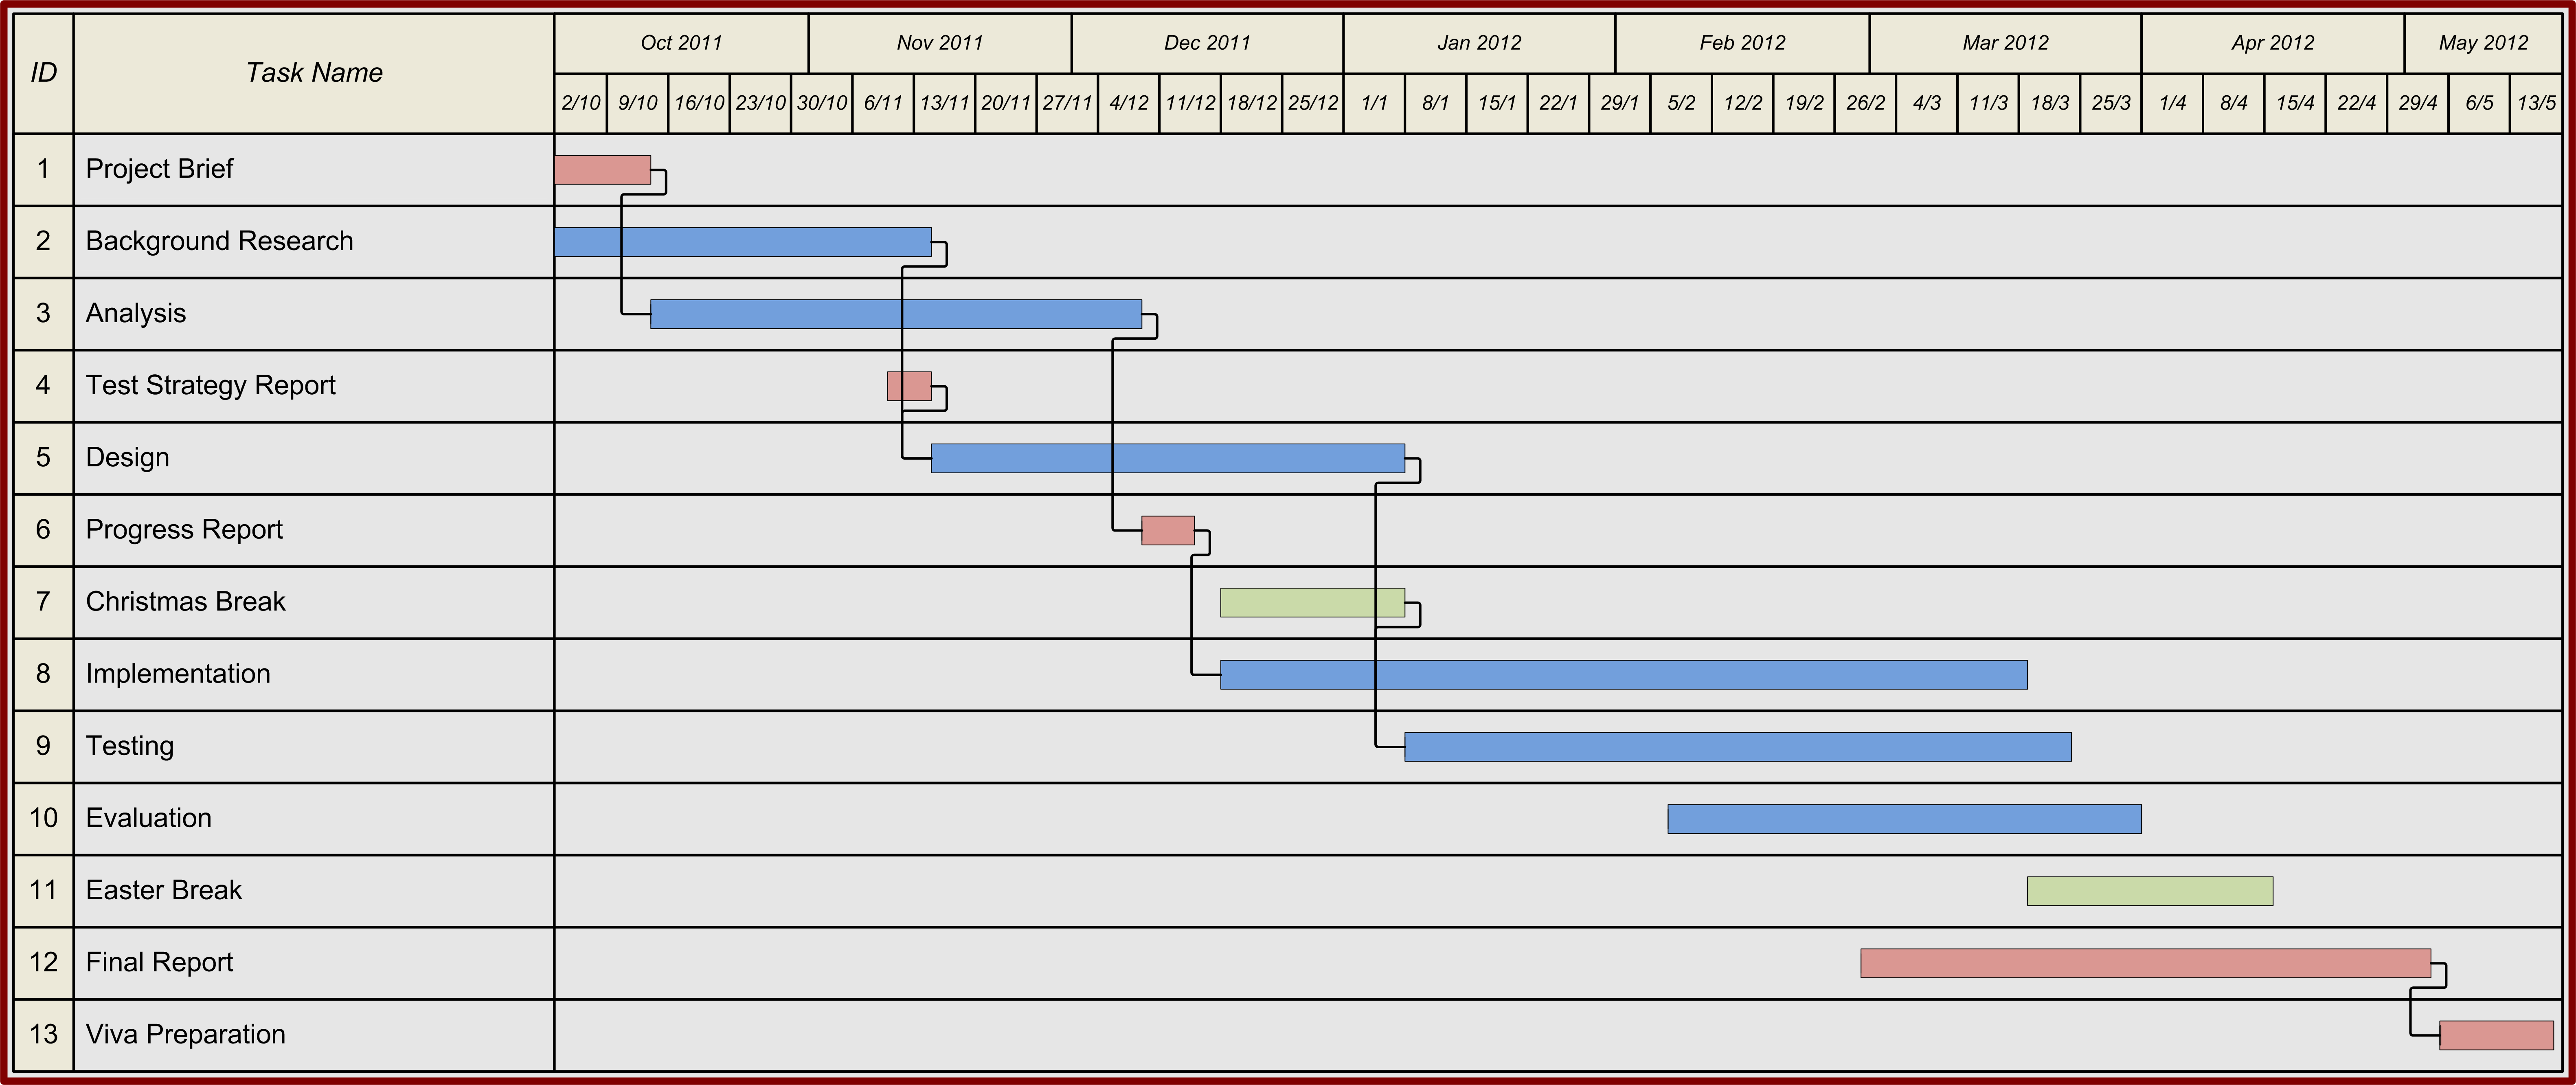
\includegraphics[scale=0.75]{img/3yp-gantt.png}
\caption{Initial Gantt Chart}
\label{fig:chart-1}
\end{figure}
\end{landscape}
\clearpage
\begin{landscape}
\begin{figure}[htb]
\centering
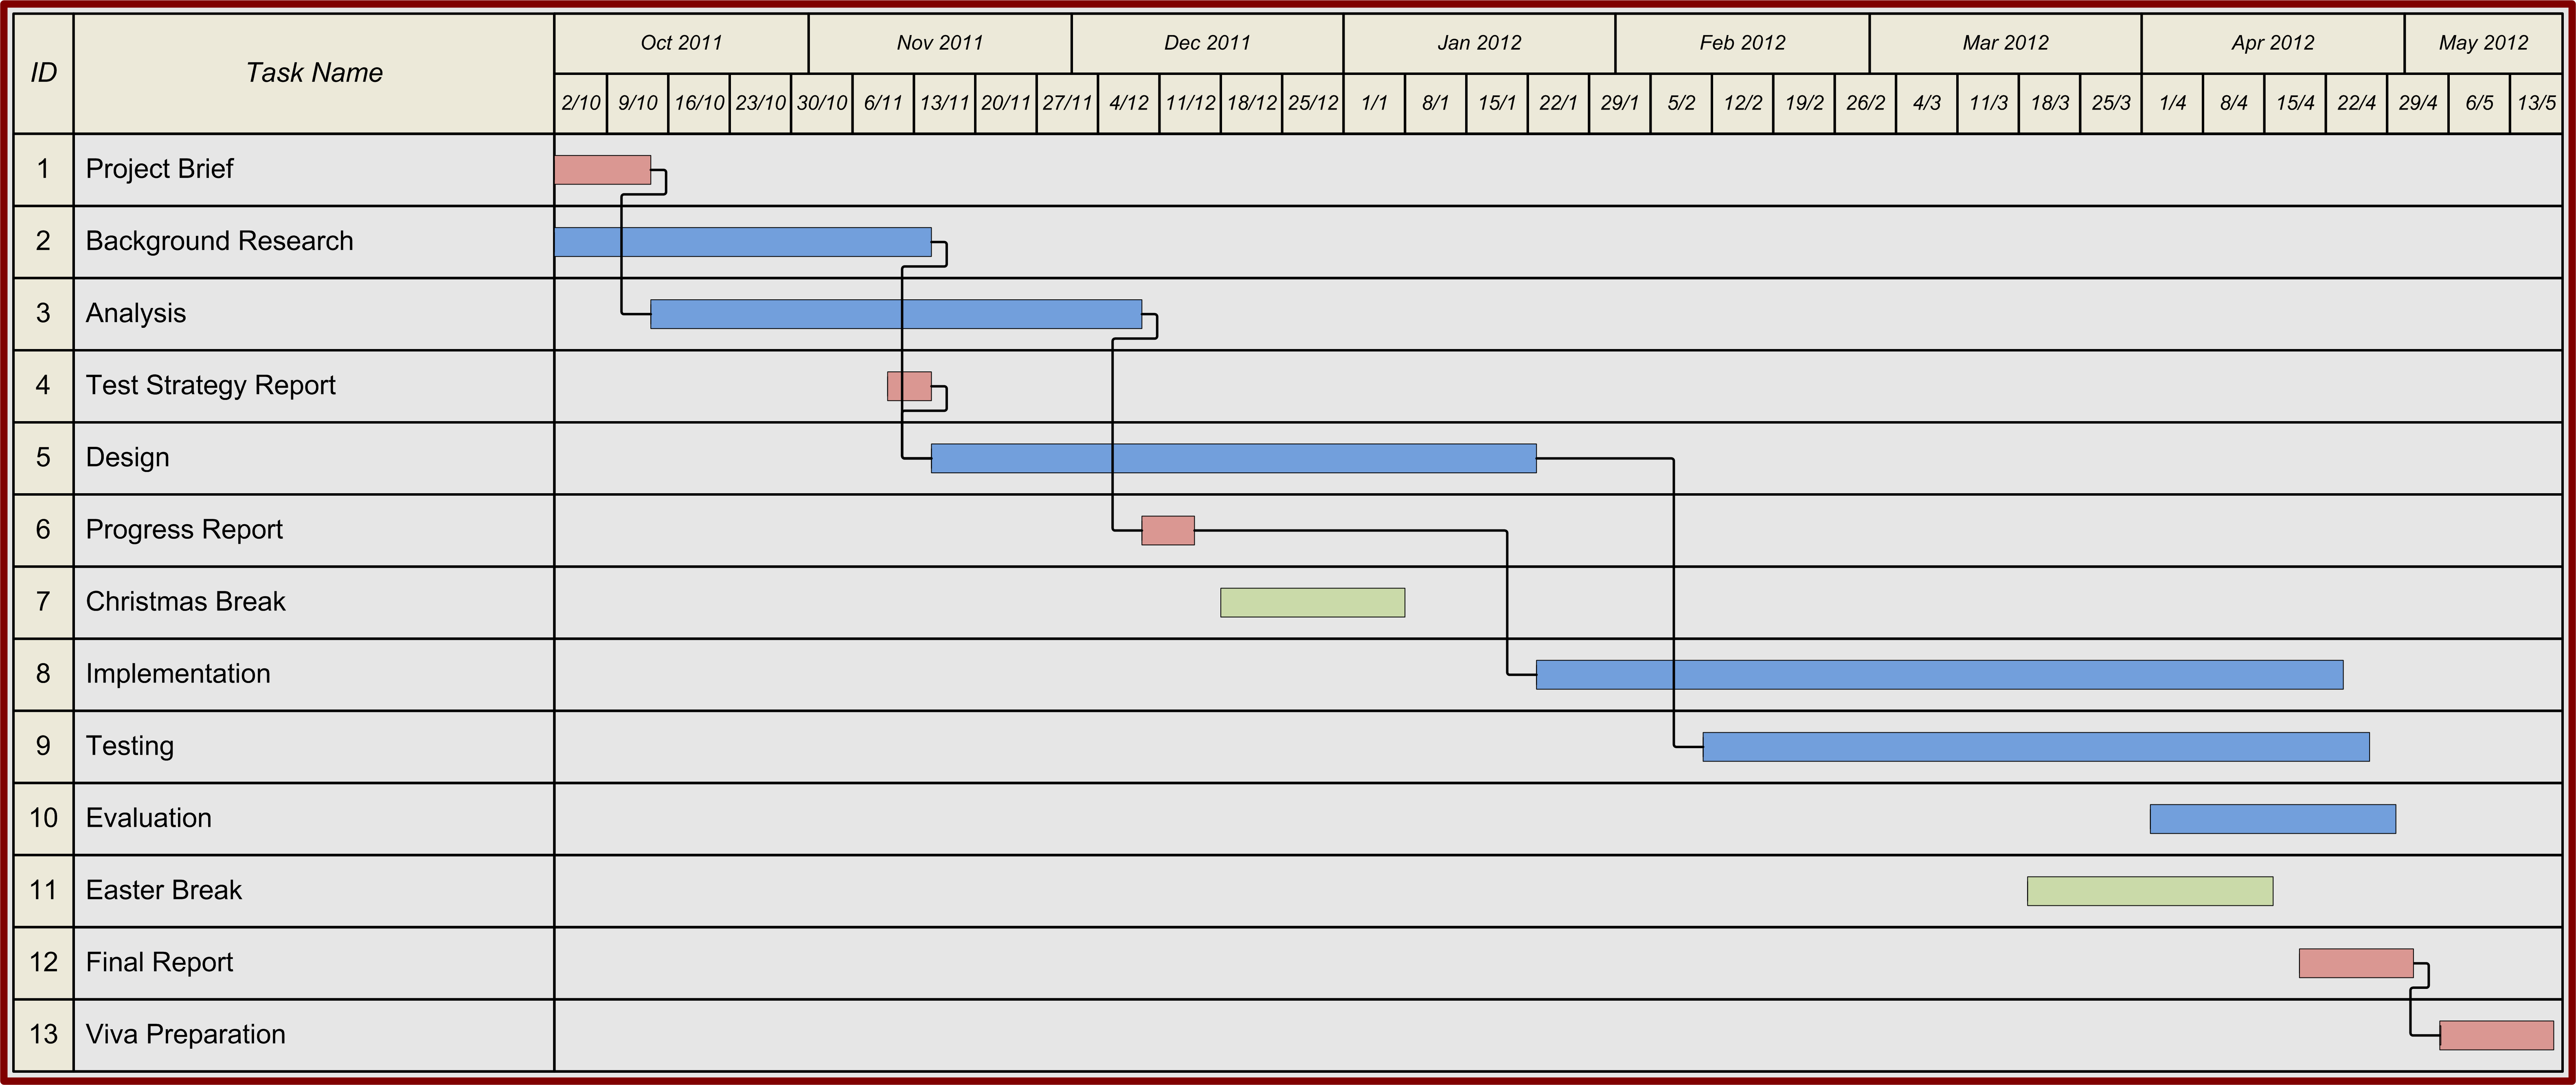
\includegraphics[scale=0.75]{img/3yp-gantt-final.png}
\caption{Final Gantt Chart}
\label{fig:chart-2}
\end{figure}
\end{landscape}

